\documentclass[11pt]{article} 
\bibliographystyle{alpha}
\usepackage[dvips]{graphicx}
\begin{document}

\title{Security Analysis of Handhelds}
\author{Vaibhav Bhandari\\
Department of Computer Science, UCSC\\
vaibhav@soe.ucsc.edu
}
\maketitle

\begin{abstract}
Handheld devices have acquired a lot of corporate as well as personal importance. They are used for variety of operations which require more security than they provide. As they lack a security framework they form the weakest link. Here we deal with two extreme examples of handhelds: Palm Pilot and the Simputer. Various security issues like passwords, access control, malicious code, protocol vulnerability, cryptography, API-level attacks, tamper resistance, memory protection and communication security are dealt with the running examples of these devices. Occasional strategies to make the devices secure are also suggested. An original authentication protocol is presented for the simputer and smart card interaction. Finally, a list of questions presented would help the reader to analysis security aspects of an Embedded system to a fair extent.
\end{abstract}

\section{Why this?}
Embedded devices form the current computing trend. Hand held devices with portability, easy access and network ability are increasingly gaining computing share. With many people using these devices, the security aspect of them warrant a more critical study. Handhelds typically have no security framework. Its not possible to build a secure application on top of an insecure one.

\section{Introduction}
The security analysis of handhelds is done in form of a study of various various critical aspects of the computing platform. The Palm OS devices form almost 80percent \cite{mudge01} of the handheld device market. The Simputer is among the genre of devices like Morhpy-one(Japan), Volks-Computer(Brazil) and Pegachu(MIT) for mass use with  text-to-speech, smart card reader, and other innovative I/O techniques. Such devices certainly promise success. Lets take closer look at what the threat is and how do we model the counter-attack.In the remaining sections the various security critical properties of handhelds are presented with running examples of these devices.

\subsection{Threat Model}
The security is designed with respect to two distinct categories of threats. One from a casual tweak and the other from a well-funded and determined crackers. The threat from latter is most but the systems by and large are designed so as to exclude the casual intrusion.

\subsection{Security Policy}
The security policy largely depends on the device usage but on generally a privilege run-level and an user run-level are essential. The security in privilege level can be classified as restricted (eg. Payroll data) or confidential \cite{pocketpc}, which requires encryption algorithms.

\section{Architecture}
Understanding the architecture of PalmOS devices and Simputer is essential to critically appreciate the underlining security features and evaluate their limitations .
\subsection{Palm Architecture}
Palm devices run Motorola DragonBall MC68328 family of microprocessors which are based on the Motorola MC68EC000 core. They are low speed ranging from 16MHz to 33MHz. They have battery backed RAM to store application data and ROM for the OS. They run PalmOS which has very little security support and lack supervisor mode of running.

\begin{figure}[h]
\centerline{
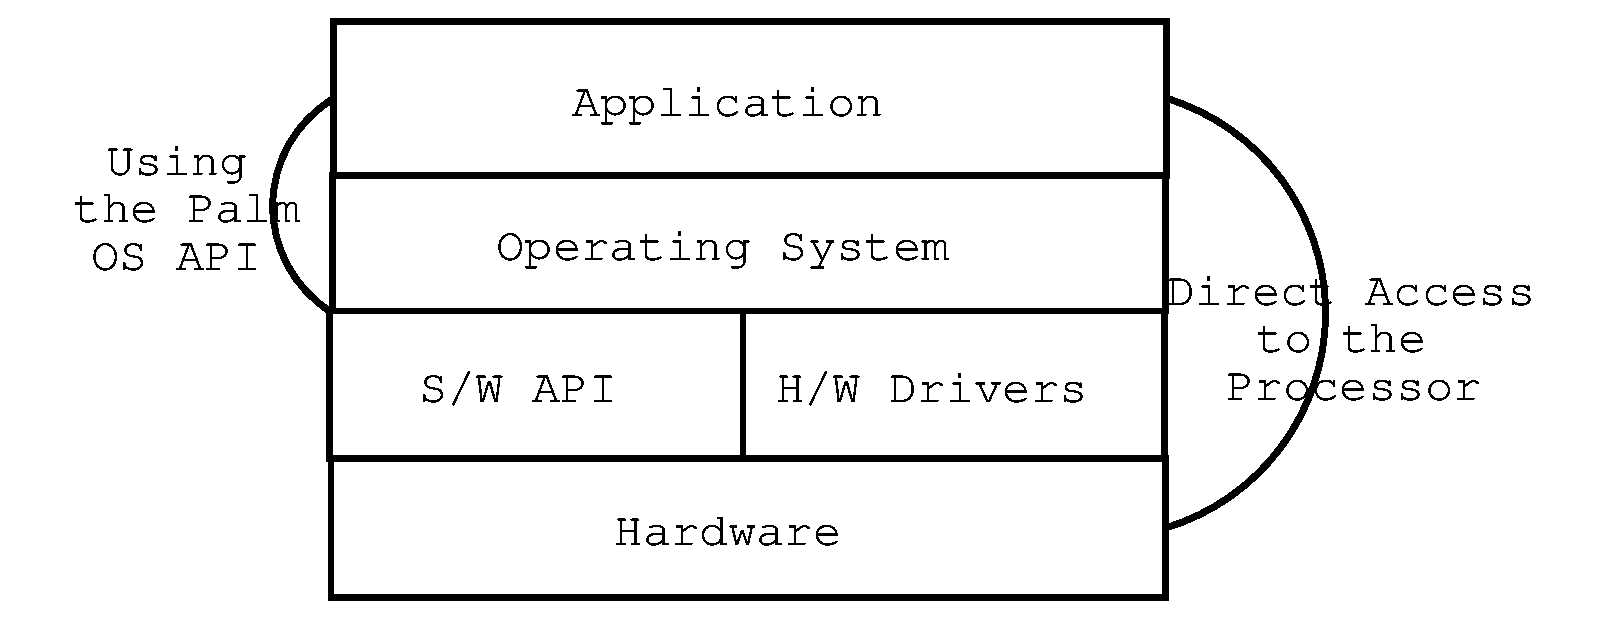
\includegraphics[width=3.2in]{palmarc.eps}
}
\caption{Typical Layered Architecture Of PalmOS device\cite{mudge01}}
\end{figure}

The Palm OS has layers: Application, Operating system and the hardware. The application can access the hardware very easily circumventing the OS. For eg to use the color LCD when the OS didn't support any. This Implies that very limited access control can be provided.

The application are generally single threaded, event driven programs. They can use a launch code to request that another application perform an action or modify data.

\subsection{Simputer Details}
The simputer on the other hand is a low-cost, multi-lingual, mass access device, currently under development\cite{simpSC}. It runs on the Intel StrongARM processors.

Information Markup Language is the primary format of the content accessed by the Simputer. Hence the  specification of IML is intimately tied to the system architecture of the Simputer and its application environment.

The Simputer has following features:
\begin{itemize}\addtolength{\itemsep}{-0.5\baselineskip}	
\item (320x240) LCD panel which is touch enabled. 
\item speaker, microphone and a few keys. 
\item soft-keyboard. 
\item stylus as the pointing device. 
\item smart card reader
\end{itemize}
 
Simputer runs {\bf Linux}. It is designed so that Linux has to be started up infrequently (at the time of battery change for example), but otherwise its in a low power mode. When its 'powered on', the user is presented with a screen having several icons (similar to the Palm home screen). Its aimed for following use: 
\begin{itemize}\addtolength{\itemsep}{-0.5\baselineskip}   
\item Information access. 
\item Computation. 
\item Transaction processing. 
\item Internet access. 
\end{itemize}

The Simputer is meant to be a shared device, shared between members of a family, or shared in public places like phone booths, shops and banks and other establishments. For this reason, and for the reason that there is no hard disk or other long term storage media on the simputer, the smart card is conceived as the personalizing agent. That is an individuals personal information is securely carried in a smart card, and then this information will be introduced into the simputer during a user session. At the end of the session, all traces of the data from the smart card are deleted so that the personal information is secure \cite{simpSC}.

\section{Security Analysis}
Security Analysis is evaluating the robustness of security policy to handle the various threats and  making certain the robustness of various security mechanisms and understanding there limitations.
\subsection{Password Retrieval}
The users of portable devices have no keyboard and require character input with a pen, so many times the users have very short passwords. Convenience gives way to gullibility. In PALM password obfuscation is weak, it gives way to XOR attack\cite{mudge01}. Password mechanism can be strengthened by: 
\begin{itemize}\addtolength{\itemsep}{-0.5\baselineskip}
\item Challenge/ Response mechanism on the network.
\item Encrypt and Salt Credentials stored on the system.
\item Implementation of {\bf power-on} password.
\item Alternative passwords like signatures, graphical passwords.
\end {itemize}

\subsection{Access Control}
Implementation of access control is be based the golden standard of authentication, authorization and audit \cite{lamp}.

The palm provides data security as individual records marked private in the applications. They are available on presenting correct password. The beaming of data can be prevented by using the {\bf beam} bit. However this comprises a very primitive and easily breakable access control. Consequently the palm-debugger can gain unauthorized system access easily. This can be relieved by logging all Palm debugger actions with time stamping for audit purpose.

In simputer access control is based on the IML access model. IML deals with the user in sessions. Each session has a database having the following format:

The session database is simply a three-column table of variable number of rows (limited by the size of the smart card and the size of the individual entries). The three columns of the table are \cite{simpIML}: 

{\bf Name or key} : This holds the name of the variable or key, an arbitrary string. 

{\bf Magic}: This column handles the access security of the variable and its value. The value of magic can be one of four possible types. 
\begin{itemize}\addtolength{\itemsep}{-0.5\baselineskip}
\item read (r): the variable can be read by anyone without a password, but to modify it requires a password.
\item exclusive (e): Password is required to read as well as write to this variable.
\item secure (s): The variable is readable by anyone with out a password, but cannot be changed from within IML environment. 
\item transient (t): variable requires password to read and write, but is not stored beyond the current session. 
\end{itemize}

Each of the four types of magic, except type s is a string starting with the single letter that denotes the type followed by a password string, that should be supplied by the user to be allowed access. For secure variables, the magic is single character 's'. 

{\bf Value}: This holds another arbitrary string that will be interpreted as the value of the variable or key named above. 
An example of a table is given below:
\begin{figure}[!h]
\begin{center}
\begin{tabular}[!h]{|lll|}
     \hline
      Name  &   Magic   &     Value \\
     \hline
     name   &   s       & Manohar \\
     address &  s       & CSA Department, IISc, Bangalore 560012\\
     DOB     &  s       & June 21 1960 \\
     Status  &  e567rty & Married \\
     phone   & ru87iii89 & 3092368 \\
     choice  & t345tyu  &  pizza \\
     \hline
\end{tabular}
\end{center}
\end{figure}
\\ The first three variables are publicly readable values. Status (married or single) being a sensitive information is accessible only through a password, in this case the string '567rty'. Since the status can change quite quickly in modern times, it is possible to modify the value after the user provides the same password. The phone number is information that is readable without a password, but needs a password (87iii89) to be modified. The last variable is the choice of food this user has made during a particular session. This value is accessible (read/write) by the production of a password (345tyu), but will not be saved beyond the current session. 
 
Any application that needs to use the data from the session database (or equivalently from a smart card) can do so by the simple expedient of using the name/key of the data item preceded by an underscore. An example IML segment that uses the database variables is given below.\\
\begin{center}
\begin{tabular}{|l|}
\hline
    \verb+<page>+\\
    \verb+ <tr><td> Name: </td><td><input type="text" width="15"+\\
    \verb+		height="1"+\\
    \verb+var="var0" value="_name" magic="s"/></td></tr>+\\
    \verb+ <tr><td> Occupation: </td><td><input type="text" +\\
    \verb+		width="15" height= 1"+\\
    \verb+var="var0" value="_occupation" magic="s"/></td></tr>+\\
    \verb+</page>+\\
\hline
\end{tabular}
\end{center}

{\bf Note}: this data can come from the smart card too!!!
IML restricts access to session DB variables to the input element. The value attribute of this element can be given a database key name (preceded by an underscore) as shown in the example above. When the browser renders the above form, the value of the name key is extracted from the database and filled in the form. 
This restriction is to ensure complete user control of the session data. Reading or writing of session data has to be at the express approval (as indicated by the correct password) of the user. In addition, transfer of such data to an application (especially an application on a remote machine) can only be through a form (input) element. The user is shown the data that will be sent to the application, and has the ability to delete or modify some fields before submitting the data.

\subsection{Malignant Code}

Malicious code like viruses is prevalent in palm mostly owing to Hot Sync operations. The malignancy can be acquired from the PC base.It can be prevented by asking the manufacturer to sign it. The required public-key cryptography implementable on these devices is through { \bf elliptic curve}, because RSA is very slow. Using Elliptic curve normal transaction such as key exchange or signature verification can be done in less than 2.4s while signature generation can be done in less than 0.9s \cite{elliptic}. The {\bf virus trigger} in Palm OS can be reduced by secure storage of entry points in a cryptographic co-processor and secure loading of applications. 

The Simputer provides the framework of IML in order to secure the applications. The secure variables do the job. Similarly system critical info can be stored on the smart card for the simputer.

Security processes must be placed at the operating system level such that they are undetectable and inescapable in order to trap malicious code \cite{mudge01}.
.
\subsection{Communication Security}
The introduction of wireless connectivity such as IEEE 802.11 wireless Ethernet1 or the Bluetooth short range radio system2 have opened more avenues of attack \cite{pocketpc}.

The  Palm IR functionality (beaming) creates a viable conduit for propagation of malignant code. The RF functionality (wireless) in Palm is by radio modem (connected to palm.net) and in simputer by a soft-modem (28.8Kbps) to a T1 line. Contagious code can be avoided by cyrptographic code signing of applications. The keys kept on Smart cards / secure digital external memory.

\subsection{Memory Protection}
The essential point is that each domain must have its own address space for enabling protection \cite{lamp71}. In absence of paging and segmentation each domain will have to have private memory.

Palm has no protection mechanism against flash memory attack owing to its memory design \cite{mudge01}. However the entire system data can be kept in an encrypted form to avoid malignancy \cite{pocketpc}.

\subsection{Smart Cards}
In an increasing networked environment many applications with intermittent connectivity must maintain much of their security state locally \cite{rosstalk}. Smart Cards are a very viable option for this use. Hence we must explore the robustness of these secure storage processors.

A complex attack on smart cards includes  \cite{ross01}.
\begin{itemize}
\item Invasive attack on Hardware: As described in \cite{ross01} all sorts of tampering techniques can be used by capable and determined  opponents with proper financial support to get hold of sensitive data from the card. Moreover discoveries like scanning capacitance microscope can fuel low-cost attacks.
\item Non-invasive hardware attack: like analysis of power consumption will fade away due to counter attacks like randomized clocking.
\end{itemize}

{\bf API Level Attacks}: Are an interesting genre of attacks on smartcards.A set of valid processing commands are chained in such a way to get access to the cards key \cite{bond01}.The attacks typically of timing, in-middle and data repeat types (using X-OR like vulnerabilities) but on processing level. This seems a low-strength dangerous attack, as the other attacks on the smart-cards involve fairly complex tampering strategies.

\subsection{Protocol Issues}
Its very difficult to design protocols for security usage. Large research has been done in this but still designing in new scenario and for new systems  always comes with interesting vulnerabilities.

How does the simputer authenticate the smart card and vice-versa? As the device is nascent their has been no solution to my knowledge. Here I propose the following authentication of the smart-card(SC) and the device(D) based on GSM mobile phone system\cite{ross01}. Note that simputer support PGP-like public key cryptography security mechanism in general and it may have more than one users and corresponding data areas. The key computations are done by Smart Card (as Crypto Processor).

\begin{enumerate}\addtolength{\itemsep}{-0.5\baselineskip}
\item For each user the smart has a separate data area one highly secure with users sensitive information and pin.
\item The user presents its pin(PIN) to the device. The device gives it to smart card which authenticates the users.
\item Once the user is authenticated(User Valid) the device must be authenticated to be able to read sensitive information from the smartcard.
\item The device sends its name(serial number $D_SN$) encrypted in its public key($K_PD$). The smart card sends this with a nonce(N), name of device and  users public key($K_PU$) all encrypted in users private key($K_SU$) to the certifying server(CA). Along with users plain text public key to the device which forwards it to the authenticating server. 
\item The authenticating server sends the authentication (GoodD or the Nonce N) encrypted in users public key. Thus the smart card authenticates the device.
\item To make the process faster the smart card also keeps a cache of authentic device key , serial number and expiration time stamp.
\end{enumerate}

The protocol:

\begin{center}
\begin{tabular}{|lll|}
\hline
 & & \\
U & $\Rightarrow $ & $ SC: PIN $ \\
SC & $\Rightarrow $ & $ D: User Valid $\\
D & $\Rightarrow $ & $ SC: K_{PD}, D_{SN}$ \\
SC & $\Rightarrow $ &  $ D: \{N, SC, K_{PD}, D_{SN}\}_{K_{SU}}, K_{PU}$ \\
D & $\Rightarrow $ & $ CA: \{N, SC, K_{PD}, D_{SN}\}_{K_{SU}}, K_{PU}$ \\
CA & $\Rightarrow $ & $ D: \{Good D\}_{K_{PU}}$ \\
D & $\Rightarrow $ & $ SC: \{Good D\}_{K_{PU}}$ \\
 & & \\
\hline
\end{tabular}
\end{center}

In {\bf BAN} \cite{abadi} Logic:
\begin{center}
\begin{tabular}{c}
(SC believes good User) and (SC believes CA said good Device)\\
\hline
SC believes good Device \\
\end{tabular}
\end{center}

\subsection{Miscellaneous Issues}
{\bf Outdated Information}: Typically handhelds have very limited storage, so most data is stored on the server. It may happen that security essential information on the server may be required or the information on the device is {\bf outdated} hence a robust and timely syncing mechanism must be incorporated. Care must be taken to eliminate any malignant code contamination. Palms HotSync is good mechanism but at times malicious, perhaps some secure web-servers can be used through IML in Simputer and through {\bf web-clippings} in Palm.\\
{\bf Audit Mechanism}: The secure applications in real world must have an audit trail, so as to assess investigation if anything goes wrong. Simputer provides the traditional Linux log tools while audit software can log Hot Syncs of Palm with a PC.\\
{\bf Business Processes}: At most times security violation happen due to holes in business processes. Hence its important that the applications run on the devices and the business processes undergo a careful analysis with respect to security.

\section{Conclusions}
Here I presented the general threat model for handhelds and corresponding security policy. Various security components were evaluated with respect to Simputer and PalmOS devices. Passwords are the mainstay of the security hence they must be implemented carefully and perhaps in non traditional way. The access control can be done innovatively according to the needs of the device as in Simputer. Malignant code can be checked with secure loading and digital signatures. Memories of these devices must be  non-tamperable hence proper security must be incorporated in the hardware. New communication techniques pose an array of Security threats for which appropriate solutions must be designed. Protocols are designers nightmare constantly posing new vulnerabilities, we can learn a lot from previous failures. Smart cards seems to offer a trusted computing base ({\bf TCB}) and secure storage for some security critical operations along with added bonus of personalizing!

Many embedded devices are presented in the market without evaluating the security aspects. Many security issues dealt here though not exhaustive can serve to evaluate an embedded system holistically to a fair extent. Here is a list of questions for analysing a device's security:
\begin{itemize}\addtolength{\itemsep}{-0.5\baselineskip}
\item Does it have a power-on password and is the password verification robust?
\item Is there access control for local/ remote operation?
\item Is there a way to check Malignant programs?
\item Is Strong Encryption available for both wired and wireless links?
\item Is Memory properly secured?
\item Is there a cyrpto-processor and how vulnerable is it?
\item Are the device protocols time/ tool tested?
\item Is there any audit mechanism available?
\item Does the device have access to updated information?
\item Finally, how benign are the business processes running on it?
\end{itemize}

\section {Acknowledgments}
Thanks every one, especially Prof. Martin Abadi and KS Vivek of PicoPeta Simputers for support and ideas.

\pagebreak[4]
\bibliography{mybib}

\end{document}
